\chapter{Opis sustava i tehničkih zahtjeva}

\section{Precizna poljoprivreda}

S ubrzanim porastom svjetske populacije, užurbano raste i potražnja za hranom. Kako bi se zadovoljila sve veća potreba, poljoprivreda se postepeno razvijala tijekom desetljeća. Brza urbanizacija svijeta dovela je do toga da 55\% svjetske populacije živi u urbanim područjima, uz značajan porast u Aziji i Africi. Do 2050. godine očekuje se da će 2,5 milijardi ljudi živjeti u gradovima. Ovo urbano širenje postavlja izazove za sigurnost hrane i prehranu, kao što su udaljenost između proizvodnih područja i potrošača, problemi s prijevozom, nagle promjene cijena te klimatski utjecaji. Kako bi zadovoljila sve veću potražnju za hranom, poljoprivreda mora povećati proizvodnju, ali je suočena s preprekama poput degradacije prirodnih resursa, gubitka bioraznolikosti i širenja bolesti. Poljoprivrednu produktivnost treba poboljšati kroz nove tehnologije, politike i bolje upravljanje prirodnim resursima \cite{modern_challenges}. 

Tradicionalnu poljoprivredu karakterizira posjedovanje vrlo malo tehničkog znanja za obradu zemlje i vrlo niska uporaba tehnologije. Ovaj način obrade poljoprivrednih površina gdje manualni rad ima glavnu ulogu donosi vrlo male prinose, primarno onima koji obrađuju zemlju. Proizvodnja ovisi o fizičkim mogućnostima poljoprivrednika, a strategije koje se koriste za obradu temelje se na tradicionalnim znanjima. Zbog niske tehnološke razine i ograničenih resursa, poljoprivrednici se za uspjeh proizvodnje oslanjaju na prirodne biološke procese i organizme koji obavljaju razne ekološke funkcije. Tradicionalne poljoprivredne prakse naglašavaju lokalizaciju, bioraznolikost, zajedničke genetske resurse i kulturno uvažavanje mnogih različitih usjeva. S druge strane, moderna poljoprivreda stavlja naglasak na proizvodnju, kapitalnu dobit, intenzitet prinosa i konzistentnost usjeva. Koristi razna tehnološka poboljšanja kako bi se postigla učinkovitija proizvodnja. Uvođenju tehnoloških inovacija u poljoprivredne procese, resursi poput vremena i novca se štede i postiže se veća količina i kvaliteta proizvodnje. Upravo visoki proizvodni kapacitet definira modernu poljoprivredu kao odgovor na rastuće potrebe ljudi i tržišta. Primjena suvremenih tehnika smanjuje rizik ovisnosti o vanjskim čimbenicima poput klimatskih promjena ili radne snage \cite{trad_poljo}.

Kao nusprodukt suvremene poljoprivrede pojavila se precizna poljoprivreda. Ona obuhvaća nove tehnološke odluke koje doprinose optimizaciji poljoprivredne proizvodnje. Temelji se na uporabi satelitske navigacije, računalnih tehnologija i naprednog nadzora. Njezin je temeljni cilj napredak i povećanje broja preciznih informacija u stvarnom vremenu kako bi poljoprivrednici na temelju dostupnih informacija mogli pravovremeno i prikladno donositi odluke \cite{arapovic}. Iako je ova grana moderne poljoprivrede započela uvođenjem tehnologija globalnog pozicijskog sustava \engl{Global Positioning System - GPS} i geografskih informacijskih sustava \engl{Geographic information system - GIS}, ovdje se također ubraja detaljno meteorološko praćenje poljoprivrednih uvjeta, poput parametara temperature, vlage zraka, količine padalina, smjera i jačine vjetra \cite{digitalagro}. Za uspješnu primjenu precizne poljoprivrede potrebno je prikupiti precizne podatke, kvalitetno ih obraditi i primijeniti na proizvodnoj površini. Prikupljanje podataka s poljoprivrednog gospodarstva uključuje uzimanje uzoraka i analize tla, mjerenje atmosferskog stanja te prikupljanje podataka pomoću daljinske detekcije te GPS i satelitskih snimaka. Koriste se različiti senzori i uređaji s GPS ili bežičnom tehnologijom kako bi se točno odredila lokacija uređaja na parceli te precizna mjesta uzorkovanja. 

Integracijom precizne poljoprivrede s naprednim softverskim rješenjima ostvaruje se pojam pametna poljoprivreda. Dok precizna poljoprivreda uzima u obzir isključivo promjene koje se odvijaju na poljoprivrednom gospodarstvu, pametna poljoprivreda koristi i kontekst okoline potaknut događajima u stvarnom vremenu \cite{arapovic}. Koncept pametne poljoprivrede uključuje predviđanje i učenje na podacima, kao i pojam velike količine podataka \engl{big data}, koji se odnosi na podatke koji dolaze u sve većim količinama, većom brzinom i raznolikošću \cite{big_data}. Ovaj se rad fokusira na mogućnosti koje nudi precizna poljoprivreda te mogućnost integracije platformi i uređaja koje omogućuju napredno nadziranje poljoprivrednih površina. 

Precizna poljoprivreda nudi niz rješenja koja olakšavaju svakodnevni rad na gospodarstvu. Problem zahtjevnog fizičkog održavanja može se riješiti automatizacijom ručnih provjera koje će mjeriti željene parametre. Neprecizna procjena količine vode potrebna za rast usjeva otklanja se korištenjem senzora za praćenje volumetrijskog sadržaja vode u tlu. Nadalje, praćenjem klimatskih promjena korisno je za određivanje idealnih vremena za sađenje i zalijevanje, kao i za predviđanje pojave štetnika \cite{iotnet_usecase}. Gledano na globalnoj skali, precizna poljoprivreda može ublažiti problem porasta zahtjeva za hranom. Istraživanje koje je provelo Europski parlament \cite{eu_study} pokazalo je kako precizna poljoprivreda može značajno poboljšati sigurnost hrane optimizacijom prinosa usjeva i omogućavanjem sigurnih metoda u proizvodnji hrane. Nadalje, promiče održivije metode uzgoja učinkovitim korištenjem resursa, smanjenjem otpada i minimiziranjem utjecaja na okoliš. Isto tako, studija tvrdi da će usvajanje precizne poljoprivrede potaknuti značajne društvene promjene, zahtijevati nove vještine i potencijalno mijenjati tržišta rada u poljoprivrednom sektoru. Implementacija tehnologija precizne poljoprivrede također zahtijeva učenje novih vještina i prilagodbu naprednim tehnološkim alatima, što produbljuje vještine stanovništva. Studija naglašava efikasnost precizne poljoprivrede zbog koje se pojedini poljoprivredni procesi mogu u potpunosti automatizirati i tako poboljšati produktivnost te smanjiti troškove rada. Stavljen je također naglasak na odluke vođenim podacima \engl{data-driven decision making} koje su potaknute redovitim prikupljanjem i analizom podataka. Istraživanje ističe i regionalni razvoj kao posljedicu usvajanja precizne poljoprivrede jer se njome potiče regionalna samodostatnost i konkurentnost prilagođavanjem poljoprivrednih praksi specifičnim regionalnim uvjetima i resursima.

U sklopu rada \cite{arapovic} provedena je istraživačka anketa nad mladim poljoprivrednicima u Hrvatskoj, odnosno nad poljoprivrednim djelatnicima mlađim od 40 godina. Cilj istraživanja bio je utvrditi upoznatost mladih poljoprivrednika s karakteristikama i primjenom pametne odnosno precizne poljoprivrede. Anketa je pokazala da je 72\% poljoprivrednika upoznato s pojmom precizne poljoprivrede, no samo jedna četvrtina ispitanika koristi preciznu poljoprivredu na svom gospodarstvu. Najviše raznovrsnih modernih tehnologija koriste poljoprivrednici koji se bave ratarstvom. 60\% ispitanika smatra da im tehnologija pomaže kod rada na gospodarstvu te se najviše koriste pametnim telefonom. Ispitivala se također uporaba tehnologije koja se odnosi na promjenjive doze aplikacije sredstva \engl{variable rate technology - VRT}, što je pokazalo da otprilike 10\% ispitanika koristi senzorske tehnologije promjenjivih doza aplikacije, primjerice prskalice. Pri upravljanju gospodarstva tehnologija se najčešće koristi za uzimanje uzoraka, i to 40\% ispitanika. Isto tako, ustanovljeno je kako se razine osviještenosti ne razlikuju značajno s obzirom na ekonomsku veličinu poljoprivrednog gospodarstva (EVPG). Nadalje, poteškoće u usvajanju informacijskih tehnologija povezuju se sa slabo dostupnim resursima, ponajprije brzini interneta. Više od 30\% poljoprivrednika navodi brzinu internetske veze kao glavnu prepreku ka digitalizaciji. Zanimljivo je istaknuti da tek 3\% ispitanika navodi nedostatak digitalne pismenosti kao problem, što upućuje da su mladi poljoprivrednici već korisnici modernih tehnologija. 

%Moj problematični poljoprivredni sustav. Ovdje opisati sa čim se poljopvrivrednici bore, šta im smeta, potkrijepiti to tako linkovima, onda naći rješenja koja su im pomogla i kako im IoT poljoprivreda boosta productivity i poboljšava usjeve i tako to. 

\section{Zahtjevi na sustav i opis predloženog rješenja}

U nastavku je predloženo rješenje koje uvažava problematiku održavanja poljoprivrednih površina i nudi alternativu izazovima hrvatskih poljoprivrednika. Sustav za udaljeni nadzor u poljoprivredi treba omogućiti praćenje parametara poljoprivredne površine u stvarnom vremenu. Da bi se to postiglo, potrebno je na površinu postaviti uređaj s primjerenim senzorima te omogućiti bežično slanje očitanih senzorskih mjerenja u stvarnom vremenu u računalni oblak. Sustav isto tako ne smije prekinuti rad ni pri gubitku internetske veze. Odabrana je arhitektura gdje se mikrokontrolerski razvojni sustav s priključenim senzorima koristi za mjerenje parametara, a putem ugrađene podrške za bežično povezivanje na Wi-Fi šalje podatke prema oblaku. Isto tako, odabran je računalni oblak koji nudi obradu podataka i njihovu trajnu pohranu te vizualizaciju, kao i pohranu posljednjeg poznatog stanja sustava.

Prilikom odabira razvojnog sustava potrebno je paziti da ima mogućnost bežičnog povezivanja putem Wi-Fi mreže. Također je važno odabrati prikladan skup senzora koji prate uvjete nužne za održavanje poljoprivredne površine. Za računalni oblak potrebno je odabrati platformu koja može progutati i obraditi veliku količinu podataka te ih zatim pohraniti. Veliku ulogu također ima sposobnost praćenja posljednjeg poznatog stanja sustava. Isto tako, potrebno je omogućiti jednostavno uspostavljanje komunikacije između mikrokontrolerskog razvojnog sustava i odabrane platforme. U oblaku je također bilo potrebno izraditi web aplikaciju koja mora korisniku pružiti jednostavnu vizualizaciju pohranjenih podataka. Glavna uloga aplikacije jest prikazati podatke i tako korisniku omogućiti udaljeno praćenje poljoprivrednih uvjeta kroz vrijeme. 

Za potrebe ovog rada odabran je razvojni sustav ESP32-C3-DevKitM-1 jer zadovoljava postavljene zahtjeve i ima mogućnost jednostavnog razvoja programske potpore korištenjem ugrađenih biblioteka. Na razvojnom sustavu nalazi se modul ESP32-C3 koji ima ugrađeno sučelje za povezivanje putem Wi-Fi mreže. Kao računalna platforma u oblaku odabran je sustav Amazon Web Services (AWS) jer nudi lako skalabilnu obradu podataka, kao i baze za njihovu pohranu. Platforma također omogućava praćenje posljednjeg poznatog stanja sustava. Za web aplikaciju odabrana je višeplatformska aplikacija Grafana koja pruža različite vrste vizualizacija, čime se poboljšava korisničko iskustvo pregleda podataka. Aplikacija također podržava alarmiranje korisnika o neželjenim uvjetima. Blok shema sustava prikazana je na slici \ref{fig:shema}. U nastavku rada opisani su svi aspekti programskog rješenja razvijeni u okviru rada, odnosno programska potpora za mikrokontrolerski sustav, kao i potpora za oblak.

\begin{figure}[ht]
	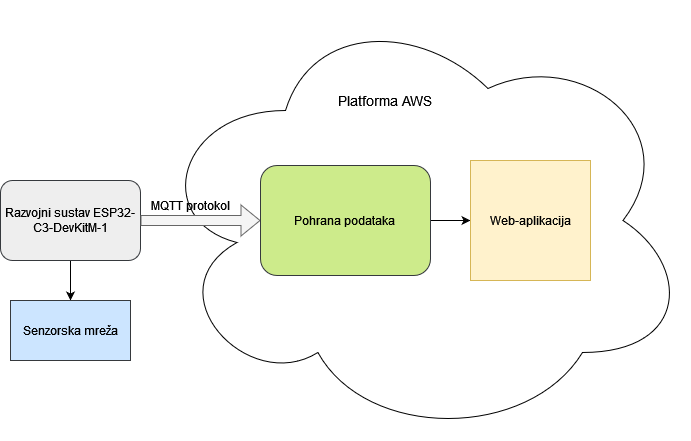
\includegraphics[width=\linewidth]{imgs/shema}
	\caption{Blok shema sustava}
	\label{fig:shema}
\end{figure}

\eject
